\chapter{Foundations in chemistry}
    This chapter acts as a bridge between A level and GCSEs. It is quite       simple with a lot of practice of molar equations, percentages and           remembering through rote learning.
    

\section{Fundamentals in chemical semantics 2.1.1}
	\paragraph{Isotopes} are the same elements (same number of protons/atomic number), but with a differing numbers of neutrons. This gives it a different mass number.
      
	Chemists compare the masses of subatomic particles using relative masses.
	This is where where we look at the mass of these particles relitive to $\frac{1}{12}$ the mass of $^12$C
	
\begin{tabular}{ |p{3cm}||p{3cm}|p{3cm}|p{3cm}|  }
 \hline
 Particle    & Abbreviation &Relative charge&Relative mass\\
 \hline
 Proton   & p+    &1+&   1\\
 Neutron& n  & 0   &1\\
 Electron& e-  & -1& 0.0005\\
 \hline
\end{tabular}

\paragraph{Charge} comes from atoms, or molicules, wich are defficient in, or have a surplus of electrons.
Given that protons have a charge of +1 and electrons have a charge of -1 to have zero overall charge we need the same number of electrons as there are nutrons, this is the most stable state.

\paragraph{Atomic Numbers}show the number of protons in an element. These are then used to order the elements in the periodic table. For example, $_{2}$Li or $_{8}$O.

\paragraph{The Mass number} is the number of protons + number of neutrons. The \textbf{atomic number} is the \textbf{number of protons} only.
An ion is a charged atom i.e. lost or gained electrons.

\paragraph{The Relative isotopic mass}is the mass of an isotope compared to \(\frac{1}{12}th\)\\ of a carbon-12 atom. In questions assume this is equal to the mass number.

\paragraph{The relative atomic mass}is the \textbf{weighted mean} mass of an atom relative to  \(\frac{1}{12}th\)\ the mass of a carbon-12 atom. The weighting takes into account \textbf{percentage abundance and relative isotopic mass}. 

\paragraph{To determine} percentage abundance and relative isotopic mass of an element, they are found experimentally using a mass spectrometer. You do not need to know how it works, but if you want, it's mentioned in the OCR A chemistry textbook.
\[m/z= \frac{Relative Mass Of Ion}{Relative Charge}\]\
\paragraph{The relative isotopic mass} is found on the x-axis and percentage abundance by the peak e.g. if there is 75.78\% of CL-35 and 24.22\% of Cl-37, you would do this:
\[Relative Atomic Mass=\frac{(75.78*35)+(24.22*37)}{100}\]\
Where 75.78x35 is the contribution from Cl-35, 24.22x37 is the contribution from Cl-37 and 100 is the max percentage. Questions like to ask you to guess what the elementn is by its mass, so make sure you are confident in this skill. 
\paragraph{For simple molecules}, the term relative molecular mass will be used.
For compounds with \textbf{giant} structures, the term relative formula mass will be used.
\section{Compounds, formulae and equations 2.1.2}
\begin{tabular}{ |p{3cm}||p{4cm}||p{3cm}||p{3cm}|  }
 \hline
 +1    & 1- &2-&3-\\
 \hline
 Ammonium \[ NH_4^+ \]    & Hydroxide \[OH^-\]    &Carbonate \[CO_3^ 2-\]& Phosphate \[PO_4^ 3-\]\\
 N/A& Nitrate \[NO_3^-\]  & \[SO_4^{2-}\]  & N/A\\
 N/A& Nitrite \[NO_2^-\]  & Sulphite \[SO_3^{2-}\]& N/A\\
 \hline
 N/A & Hydrogencarbonate \[HCO_3^-\] & Dichromate(VI) \[Cr_2O_7^{2-}\] & N/A\\
 \hline
 N/A & Manganate(VII)/ Permanganate \[MnO_4^-\] &N/A&N/A\\
 \hline
\end{tabular}
\section{Amount of substances 2.1.3}
\subsection{1.The mole}
\paragraph{The amount of substance},n, is used to count the number of particles in a substance- measured in moles. One mole contains \textbf{\(6.02*10^{23}\)} particles- known as \textbf{Avogadro's constant}.
\paragraph{Molar mass} /\(M_r\) is the mass per mole which is why its units are \(gmol^{-1}\) e.g. carbon has a molar mass of 12, where 1 mole is 12 grams.
\newline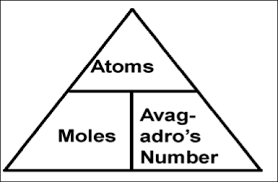
\includegraphics[scale=1.0]{atms_triangle}
\paragraph{A mole of gas} fills, in standard conditions (RTP), 24.0 dm3 of space. The number of moles is directly proportional to the space filled. You can find this information on the formula sheet under “Molar gas volume”.
\paragraph{When the substance isn’t under standard conditions} the ideal gas equation is used, \(pV=nRT\). They give us a number called the Gas constant- 8.314 J/mol/K. This value is given on the formula sheet, however you have to know non-SI units and working it out takes longer than remembering this figure.
\subsection{2.The determination of formulae}
\paragraph{Empirical Formula} is the simplest whole number ratio of atoms of each element present in a compound.
\paragraph{Molecular formula} is the number and type of atoms of each element in a molecule e.g. \(H_2SO_4\) .
\paragraph{The determination of formula} is a necessary part of this exam. They love questions along the lines of:
\begin{enumerate}
\item “Raheem has found that his substance has a composition by mass of  23.3% magnesium, 30.7% sulfur and 46.0% oxygen "
\begin{itemize}
\item (a) Work out the empirical formula
\end{itemize}
\end{enumerate}
\paragraph{It is assumed} that the percentage composition of the element is equal to the mass of the element e.g. 23.3\% is 23.3g. We also know the \(M_r\) of each element:
\begin{itemize}
\item Magnesium is 24.3 \(gmol^{-1}\)
\item Oxygen is 16 \(gmol^{-1}\)
\item Sulfur is 32.1 \(gmol^{-1}\)
\end{itemize}
\paragraph{Next, you find the moles} by dividing the mass by the \(M_r\). 
\newline Therefore:\(\frac{23.3}{24.3}\) = 0.959, \(\frac{30.7}{32.1}\) = 0.956 and \(\frac{46.0}{16}\) =2.875. Then you divide by the smallest number of moles, giving the empirical formula. 0.959/0.956=1, 0.956/0.956=1 and 2.875/0.956=3. This makes the empirical  formula: \(MgSO_3\) .
\paragraph{In other cases}, they may ask you tork out the molecular formula using the empirical formula and the molecular mass given in the question. For example:
"Fatima found that a substance had a percentage composition of 40.0% carbon, 5.7% hydrogen and 53.3% oxygen has an atomic mass of 175 g/mol. What is the molecular formula?"
\paragraph{To minimise my working,}I shall provide you with the empirical formula \ch{CH_2O}. You can try to work out how I did this using the method above.
\paragraph{In order to work out the molecular formula} you need a little algebra. As we know the Mr is 180 and the empirical formula is \(CH_2O\) - Mr 30,as we want to work out the number of each atom you would do:
\newline \[180=30x\] \[\Delta\\x=6\]
\paragraph{Finally,} you multiply the atoms present in the empirical formula by 6 from the above equation. This gives a molecular formula of \(C_6H_{12}O_6\) .
\paragraph{Hydrated salts} are calculated in much the same way. They are expressed
like this CuSO4·nH2O and you will be given some numbers to workout n.These are likely the mass of water and mass of anhydrous salt .
\newline Heating a substance removes the H2O making it anhydrous. To Hydrate simply dissolve the salt in water and evaporate the water very slowly.(see pg.24 in book).
\subsection{How accurate is experimental formula?}
\paragraph{You need to make an assumption that all water is lost}. You can only see the surface of the crystals; the inside is unknown to us, so water could be found there. To \textbf{reduce error, you should heat to a constant mass}- when mass no longer changes when heated. rthis means you can be sure that it is anhydrous.
\paragraph{You also assume there is no further decomposition}. Many salts decompose further when heated e.g. \(CuSO_4\) turns into black copper(III) oxide.
\subsection{3.Calculation of reacting masses, gas volumes and mole concentrations}
\paragraph{You need to know}all the calculations using liquids, gases and solids to find moles. You also need to know how to convert between \(gdm^{-3}\) and \(moldm^{-3}\) . You just need to remember that when you convert from \(moldm^{-3}\) you just multiply by Mr.
\newline
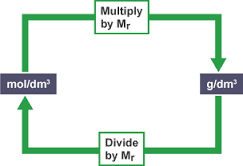
\includegraphics[width=0.85\textwidth]{chem1.png}
\newline You will also need to know how and when to use the ideal gas equation:
\begin{equation}
pV=nRT
\end{equation}
\begin{center} p= Pressure in Pa

 V= Volume in \(m^3\) 

n= moles

R= ideal gas constant(8.314 \(Jmol^{-1}K^{-1}\) ) 

T= temperature(K) 
\end{center}
\paragraph{With the ideal gas equation} you assume that: no intermolecular forces;sizes are negligible; random motion and elastic collisions.
You will also need to remember how to convert between the units as questions sometimes try to trick you. These are listed here:
\begin{itemize}
\item \(cm^3\) to \(m^3\) = \(*10^{-6}\)
\item \(dm^3\) to \(m^3\) = \(*10^{-3}\)
\item \degree C to K = +273
\item kPa to Pa = \(*10^3\) 
\item 1 atm = 101kPa = 101000 Pa
\end{itemize}
\newpage
\begin{equation}
Percentage Yield= \frac{Actual Yield}{Theoretical Yield}\\
\end{equation}
\newline
\begin{equation}
Atom Economy= \frac{\sum Mr(desired) prod}{\sum Mr All Prod}\\
\end{equation}
\paragraph{Percentage yield} doesn't really allow 100\% in real life because: the reaction \textbf{may not have fully taken place};\textbf{side reactions occur} and \textbf{purification} leads to loss in product.
\%age yield is in reference to the percentage of the theoretical yield that was actually yielded i.e. actual yield. Atom economy simply refers to the number of wasted atoms (atoms that form waist products).
\section{Acids 2.1.4}

	\paragraph{The acids to remember} are the following:
	\begin{itemize}
		\item HCl is Hydrogen Chloride
		\item \ch{H2SO4} is Hydrogen Sulphate
		\item \ch{NOH3} is Nitric Acid
		\item \ch{KOH} is Potassium Hydroxide
		\item \ch{CH3COOH} is Ethanoic Acid (although it is commonly called Acetic Acid).
	\end{itemize}
    Acids release \ch{H+} ions when in aqueous solution.
	To examine the strength of an acid we must look at the dissociation of the \ch{H+} ions.
	Take for example HCl. The dissociation of HCl in aqueous solution looks like this, 
	\begin{center}
		\ch{HCl(aq) -> H^+(aq) + Cl^-(aq)} 
	\end{center}
	As you can see all of the hydrogen atoms have dissociated.
	This would make HCl a \textit{strong acid}. 
	
	Where the \ch{H+} ions only partially dissociate we call it a \textit{weak acid}. Take Ethanoic acid, its dissociation in aqueous solution looks like this, 
	\begin{center}
		\ch{CH3COOH(aq) <=> H^+(aq) CH3OO^-(aq)}
	\end{center}
	 As we can see the \ch{H+} ions haven't entirely dissociated.
	 The \ch{<=>} implies that the reaction is incomplete and forms an equilibrium, so the acid hasn't completely dissociated.
	
	There is a point to be made that not all ionic compounds with hydrogen atoms are acids.
	It is only those compounds that form \ch{H+} ions when dissolved in aqueous solution that we call acids.
	
	\paragraph{The common bases} are metal oxides, metal hydroxides, metal carbonates and ammonia, \ch{NH4}.
	Bases neutralise an acid to form a salt.
	
	\paragraph{An Alkali} is a special type of base which, when dissolved in water, releases hydroxide ions.  They are also known as soluble bases.
	For example take the base \ch{Mg(OH)2},
	\begin{center}
		\ch{Mg(OH)2(s) + aq -> Mg^{2+}(aq) + 2 OH-(aq)}
	\end{center}
	We can see that \ch{Mg(OH)2} is an alkali as it releases \ch{OH-} ions when dissolved in aqueous solution.
	
	\paragraph{The alkali and base to remember} are the following:
	\begin{itemize}
		\item \ch{NaOH} is Sodium Hydroxide
		\item \ch{KOH} is Potassium Hydroxide
		\item \ch{NH3} is Ammonia
	\end{itemize}
    \paragraph{You need to remember} that:
   \begin{itemize}
\item\ch{H+ + OH- -> H2O}, 
\item   \ch{CO3^{2-} + 2 H+ -> H2O + CO2} 
\item   and finally \ch{O^{2-} + 2 H+ -> H2O}.
	\end{itemize} 
    Using these ionic equations you should be able to form full equations.
	
	\paragraph{Titrations} are a technique to achieve a neutralisation reaction.
	We take an acid and a alkali and we slowly add one to the other using a burette.
	
	
	The preparation of a standard solution simply involves dissolving a exact and known mass of ionic compound and dissolving it in a know volume of water.
	This is done in a volumetric flask.
    \section{Redox 2.1.5}

	\paragraph{OIL RIG} is a fantastic acronym.
	Oxidation Is Loss, Reduction is gain.
	Remembering this is vital.
	If we describe a reaction as having \textit{oxidised} X, we mean to say that X has lost electrons.
	If a reaction is described as having \textit{reduced} X, we mean to say that X has gained electrons. It is important to remember \textbf{elements have an oxidation number 0.}
	
	To write a redox reaction we have equations like this:
	\begin{center}
	\vspace{7mm}
	\ch{
		2 "\OX{o1, \ox[pos=top]{0,Na}}" + "\OX{r1, \ox[pos=top]{0,Cl}}" {}2
		->
		2 "\OX{o2,\ox[pos=top]{+1,Na}}" {}+ + 2 "\OX{r2, \ox[pos=top]{-1,Cl}}" {}-
	}
	\redox(o1,o2){\small OX: $- 2\el$}
	\redox(r1,r2)[][-1]{\small RED: $+ 2\el$}
	\vspace{7mm}
	\end{center}
	We use Roman numerals to indicate oxidation numbers, memorise the following oxidation numbers:
	\begin{itemize}
		\item Oxygen has the oxidation number -2 unless in peroxide, in which case it is -1
		\item Hydrogen has the oxidation number +1 unless in a metal hydride in which case it is -1
		\item Fluorine has the oxidation number -1
	\end{itemize}
	So to work out whether a chemical has been oxidised or reduced we do the following.
	
	\begin{enumerate}
		\item Find the balanced symbol equation,
		
		\ch{2 Al + 3 H2SO4 -> Al2(SO4)3 + 6 H2}
		
		\item Then we fill in the oxidation numbers for the ones we know,
		
		 \ch{2 "\ox{0, Al}" {} + 3 "\ox{+2, H}" {}2 "\ox{-2, SO}" {}4 -> Al2 "\ox{-6,(SO}" {}4)3 + 6 "\ox{0, H}" {}2}
		 
		\item The \ch{Al2 "\ox{-6,(SO)3}" {}4} has no overall charge so the oxidation numbers must add to 0,
		
		\ch{"\ox{+6, Al}" {}2 "\ox{-6,(SO4)}" {}3}
		
		\item Now we have \ox{+6, Al}$_2$ we can see that \ox{+3, Al}. So Aluminium went from Al to \ox{+3, Al} meaning it has been oxidised in this reaction.
		
		\item The hydrogen went from \ox{+2, H}$_2$ to \ch{H2}. This is a reduction so we say hydrogen has been reduced.
	\end{enumerate}
	\paragraph{It is important}to note that when writing oxidation numbers down in exam questions, it only means for one atom of a molecule.
    In summary oxidation numbers refer to the number of electrons individual atoms in compounds have lost/gained.
	They are like charge but apply to atoms and not the overall compound.
	They are used to explain whether a reaction has oxidised an atom or reduced it.
   \newpage
   \section{Electron structure 2.2.1}

	\paragraph{Shells} are areas where there is a high probability of finding an electron.
	They are split by looking at major energy levels.
	The period an atom is in indicates how many shells it has.
	The number of electrons that can fit into a shell can be worked out by $2n^2$ where $n$ is the shell number.
	
	\paragraph{Shells are sub-divided} into sub-shells. The ones you need to know are as follows,
	\begin{itemize}
		\item s orbital which can hold 2 electrons, one in all shells
		\item p orbital which can hold 6 electrons, one in all but shell 1
		\item d orbital which can hold 10 electrons, one in all but shells 1 \& 2
	\end{itemize}
	They fill in order.
	
	\paragraph{Orbitals} are regions around the nucleus which can hold up to two electrons with opposite spin.
	This diagram is of a P orbital and the arrows indicate the spin:
    \begin{center}
    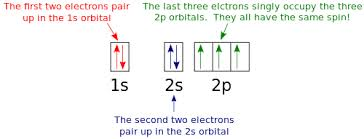
\includegraphics[scale=1]{orbital}
    \end{center}
    \paragraph{Order of fill} is as follows, 1s$^2$2s$^2$2p$^6$3s$^2$3p$^6$4s$^2$3d$^{10}$4p$^6$ in the standard format $x$s$^n$
    The examination may well ask you to write the electron configuration of an atom.
	Unless otherwise instructed, a short cut is to use a noble gas as a base.
	For example if I said write the electron configuration of sodium you can say [Ne]3s$^1$.
	You need to know how to do this for all elements up to and including Kr.
   \paragraph{Energy levels} are the reason different shells fill differently. 
   As you probably know, lower energy levels need to fill before higher ones.
   This is why,for example, the s- subshell fills before the p- subshell.
   As we go up, the shells we also ascend in energy level.
	The most interesting part is the 4s sub-shell and the 3d sub-shell.
	The 4s sub-shell and the 3d sub-shell have very similar energy levels.
	The 4s sub-shell is, however, slightly lower so the 4s fills first.
	When the 3d sub-shell fills the energy level falls meaning, the 4s fills before 3d and the 4s empties before 3d.
	This is important when looking at the electron configuration of D Block ions.
    \section{Bonding 2.2.2}
    \paragraph{Ionic bonding} is the \textbf{strong electrostatic attraction} between anions and cations.
    It usually occurs when there is a \textbf{metal cation} and a \textbf{non-metal anion}.
    \paragraph{The giant ionic lattice} is the structure of ionic compounds. 
    Each ion is surrounded by oppositely charged ions in a regular structure e.g, in NaCl , each Na$^+$ ion is surrounded by 6 Cl$^-$ ions and vice-versa.
    \paragraph{Ionic compounds have high melting and boiling points} because there needs to be high temperature in order to overcome the strong electrostatic forces between ions.
    The melting point is higher if the ionic charges are greater and the size of an ion is also a factor.
    \paragraph{Ionic compounds usually dissolve in polar solvents}such as water. Polar molecules attract and surround each ion in solution and break down the lattice e.g. NaCl dissolves in water.
    However, in ionic structure with large ionic charges, some polar solvents such as water may not be able to overcome the strong electrostatic attraction.
    \paragraph{ In a solid state, ionic structures don't conduct electricity} because the \textbf{ions} are \textbf{localised} meaning there are \textbf{no mobile charge carriers}.
    In an \textbf{aqueous state}, however, the \textbf{ions are free to move} as mobile \textbf{charge carriers} allowing electricity to be conducted.
   \paragraph{Dot-and-cross diagrams} are the same as they have always been.
	Used for drawing the simplest of ionic bonds, that of metal - non-metal.
	Just remember: the square brackets;only the outer shell is drawn and that the charge is shown as superscript.
  \pagebreak
  \paragraph{In summary} ionic compounds have these properties:
    \begin{itemize}
		\item Have \textbf{high melting and boiling points}
		\item Tend to \textbf{dissolve} in \textbf{polar} solvents
		\item Only conduct \textbf{electricity} when in \textbf{liquid} state or dissolved in aqueous solution.
	\end{itemize}
 
    \paragraph{Covalent bonding} is the strong electrostatic attraction between a shared pair of electrons and the nuclei of the bonded atoms. It occurs in:
    \begin{itemize}
	 	\item Non-metallic elements such as \ch{H2} and \ch{O2} form covalent bonds.
	 	\item Non-metallic compounds such as \ch{H2O} and \ch{CO2} form covalent bonds.
	 	\item Even polyatomic ions are covalently bonded such as \ch{NH4^+}
	\end{itemize}
    \paragraph{It can also be thought of as an overlap of orbitals} each containing \textbf{one} electron to give a shared pair of electrons. 
    This is why when drawing a dot and cross diagram for this, you draw overlapping circles with electrons shared.
    These electrons are attracted to the nuclei of both the bonded atoms.
    The bonded atoms often have the same elec. config. as the nearest noble gas.
    There are the following three types of covalent bonding that you are expected to know about,
	\begin{enumerate}
		\item Single covalent bonding, this is where there is one shared pair of electrons per nuclei.
		\item Multiple covalent bonding, this is where there are multiple pairs of shared electrons per nuclei e.g. double bond in \ch{CO2} 
		\item Dative covalent bonding, this is where the shared pair is supplied by only one of the atoms.
	\end{enumerate}
   \begin{center}
   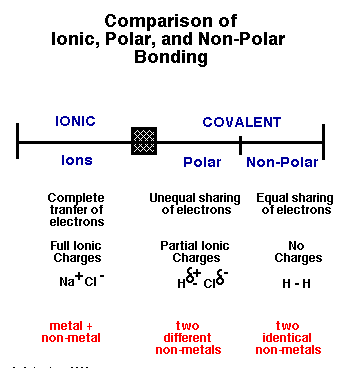
\includegraphics[scale=1]{2016-08-10}
\end{center}
   \ch{NH4^+} is a good example of a dative covalent bond. A \ch{H+} ion meets ammonia and ammonia provides the electron pair for the covalent bond.The dative covalent bond is shown by a $\rightarrow$ to the hydrogen i.e.
   \newline
    \begin{center}
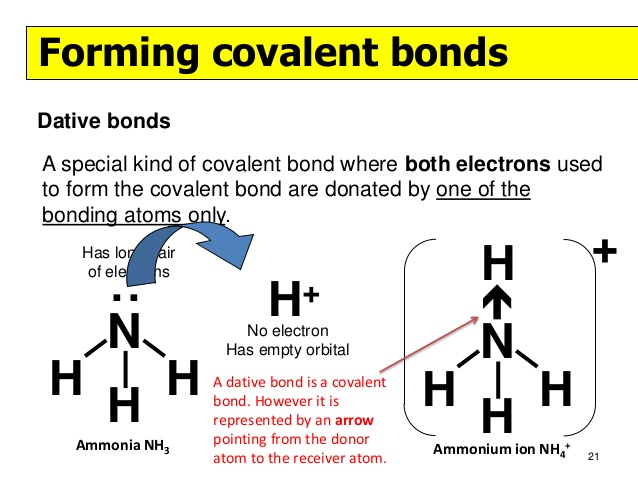
\includegraphics[scale=0.5]{ammonia}
\end{center}
\paragraph{You will need to learn}all of the types of covalent bonds. Using your GCSE or A-level textbook for any practice you require is very useful to master this skill.
	\paragraph{Average Bond Enthalpy} is simply a measure of the  covalent bond strength, take a \ch{Br-Br} \textbf{covalent} bond for example. \footnote{Note that you only need to understand the concept of avg. bond enthalpies; definitions for this are not required.}
   The larger the value of the average bond enthalpy, the stronger the covalent bond.
    \section{The shapes of simple molecules and ions 2.2.2}
	
	\paragraph{You need to know} the shapes of, and bonding angles in, molecules and ions with up to six electron pairs (including lone pairs) surrounding the central atom as predicted by electron pair repulsion.
	
	\paragraph{Electron pair repulsion} is used for explaining and predicting shapes of covalently bonded molecules as well as the relative repulsive strengths of paired and unpaired electrons.
	It works on the principle that electron pairs repel to arrange themselves around an atom as far apart as possible.
	They do this in 3D, which may sound obvious, but so far in chemistry we have worked only with 2D models.
	To draw 3D diagrams we need to understand the following standards,
	\begin{itemize}
		\item \chemfig{A-B} is used for a bond in the same plane as the paper
		\item \chemfig{A<B} is used for a bond coming out of the paper
		\item \chemfig{A<:B} is for bonds going into the plane of the paper
	\end{itemize}
    \paragraph{Lone pair} repulsion is greater than that of bond pair.
	This is because the lone pair of electrons occupy more space than the bonded pair, overall resulting in a slightly higher repulsion from the lone pair.
	The bonding angle is, therefore, reduced by around 2.5\degree for every lone pair.
	
	\paragraph{Common, and basic examples} are molecules such as, \ch{CH4} which has a bonding angle of 109.5\degree and no lone pairs and forms a tetrahedral structure; \ch{NH3} which has a bonding angle of 107\degree with one lone pair and this is pyramidal; finally \ch{H2O} which is non-linear and with its two lone pairs has a bonding angle of 104.5\degree .
	
	\paragraph{The last shapes to be familiar with} are \textit{trigonal planar} which have a bonding angle of 120\degree , \textit{linear} which are 180\degree and \textit{octahedral} which are 90\degree . 
  \section{Electronegativity and bond polarity 2.2.2}
\paragraph{Electronegativity} is the ability of an atom to attract bonding electrons in a covalent bond.	
	\paragraph{The Pauling scale} is a scale used to measure the \textit{electronegativity} of an atom. As we go right, across the periodic table, the electronegativity increases alongside a decrease in atomic radius. As we move up the table we see an decrease in the number of shells, hence a decrease in atomic radius, so we see then another increase in electronegativity. So the nearer F in the table, the higher the electronegativity.
	\paragraph{Covalent, Polar covalent and ionic} bonds are defined as the difference in electronegativity of the bonding atoms.
	Where the difference is zero we call the bond covalent/ non-polar covalent.
	Where the electronegativity difference is less than 1.8 (but greater than 0) we call it polar covalent and where it is greater than 1.8 we call it ionic.
\paragraph{Polar bonds} are covalent bonds between two elements with \textbf{unequal} electronegativities.
	\chemfig{H^{\delta +}-Cl^{\delta -}} is an example of a polar bond, and by extension a polar molecule.
	Hydrogen has a lower electronegativity than chlorine causing the chlorine in the covalent bond to become slightly negative.
	This type of bonding is called a permanent dipole.
\paragraph{Larger molecules} are interesting because we need to look at structure to see if the overall molecule is polar or non-polar(due to dipoles cancelling each other out due to their direction).
	Take \ch{H2O}, this has a non-linear structure. Both the \chemfig{H^{\delta +}-O^{\delta -}} bonds are polar and given its non-linear structure, these polar bonds don't cancel out.
	This makes \ch{H2O} a polar molecule because it has an overall \textbf{dipole- the separation of opposite charges}. It has a permanent dipole as the dipole doesn't change.
	\paragraph{However, take \ch{CO2}, a similar covalent molecule} with two \chemfig{C^{\delta +}=O^{\delta -}} polar bonds.
	But this is where it changes. The structure is linear.
	This means that the two polar bonds cancel out \chemfig{O^{\delta -}=C^{\delta +}=O^{\delta -},
	meaning that the overall molecule, in the case of \ch{CO2}, is non-polar.
    \paragraph{A bond will be non-polar when}: 
    \begin{enumerate}
\item The bonded atoms are the same- a pure covalent bond e.g. \ch{O2}
\item The bonded atoms have the same or very similar electronegativities. 
\end{enumerate}
Carbon and hydrogen have similar electronegativities- that's why hydrocarbon liquids are usually non-polar solvents and don't mix with water.

\section{Intermolecular Forces 2.2.2}
An important distinction from ionic or covalent bonding is that these are forces between different molecules rather than what holds\textit{ a molecule} together. Permanent dipole–dipole and induced dipole–dipole interactions can both be referred to as van der Waals’ forces. This is important to know if your teacher isn't aware of this change to the syllabus.

	\paragraph{Permanent dipole - dipole interactions} are caused by\textbf{ polar molecules attracting each other} and forming a permanent electrostatic interactions.
	This is quite similar to giant ionic lattices but occurs with polar covalent molecules such as water rather than ions.
	The distinction is that it is \textbf{between separate molecules} e.g. water molecules. See the example below:
    \begin{center}
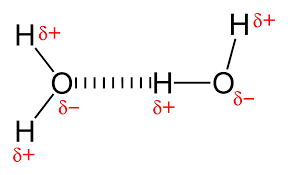
\includegraphics{permanentdipole}
\end{center}
	
	Generally permanent dipole interactions are conducive to a higher boiling point, given the \textbf{extra energy required to break the interaction.}
	
	\paragraph{Hydrogen bonding} is a special type of permanent dipole-dipole interaction. More specifically, it is ``intermolecular bonding between molecules containing N, O or F and the H atom of –NH, –OH or HF".
	
	\paragraph{Hydrogen bonding has a significant influence} on the properties of many molecules.
	Water, for example, is affected by hydrogen bonding.
	Hydrogen bonding allows for the formation of a more open lattice structure by holding the molecules further apart. The water molecules in ice are further apart than water. Therefore ice is less dense than liquid water and floats. The bond angle in hydrogen bonding is close to 180\degree , creating an open tetrahedral lattice full of holes. It also contributes to the high melting and boiling points of water.
	
	\paragraph{London Forces} are \textbf{induced dipole-dipole} interactions.
	\textbf{Electrons move randomly}, which may produce polarity in a molecule.
	This \textbf{temporary polarity} may allow the formation of an \textbf{instantaneous dipole}, which\textbf{ induces dipole on neighbouring molecules}. 	This interaction \textbf{occurs in every molecule} causing attraction between them.
	This, on a micro scale, isn't a long lasting, however when we look on a macro scale with a massive number of molecules this has a large affect.

	London forces strength is dependent on the number of electrons.
	\textbf{Elements with large number of electrons have stronger London forces} due to the \textbf{greater probability} of an interaction.
	So as we move down the periodic table we would expect a higher boiling point (where London forces are the primary interaction).
	
	\paragraph{Simple molecular lattices} are formed when a simple molecular substance
	\footnote{A simple molecular substance is one with a defined number of atoms and with defined molecular formula e.g. \ch{H2}} are in their solid form.
	They are simply put ``covalently bonded molecules attracted by weak intermolecular forces, e.g. \ch{I2}, in a simple molecular lattice structure".
	The molecules in simple molecular lattice are held together by repetitively \textit{weak} intermolecular forces. The atoms within the molecules are held together by very \textit{strong} covalent bonds.
	
	\paragraph{Solubility} of these different types of compounds follow this basic rule, in general: Polar compounds will be soluble in polar solvents and non-polar compounds will be soluble in non-polar solvents. It is important to note that most simple molecular lattices are non-polar, so are insoluble in polar solvents.
	
	\paragraph{The reason for some polar molecular compounds being soluble} in polar solvents is that the \textbf{polar solvent attracts the polar compound.}
	This attraction, in a similar way to ionic compounds, acts to \textbf{pull apart the permanent dipole-dipole} bonds and causing the compound to dissolve.
	
	\paragraph{The reason for the non-polar compounds dissolving} in non-polar solvents is much the same.
	The intermolecular interactions are the same so the solvent is able to break down the simple covalent lattice.
	
	\paragraph{Electrical conductivity} is nil for simple molecular structures.
	There are no mobile charged particles meaning that there will be no way for the substance to be conductive.
    \paragraph{They have low melting and boiling points} because they are held together by weak intermolecular forces. They are solidified by reducing the temperature low enough. When melting, the covalent bonds \textbf{do not break}.